På figur~\ref{fig:crossovertest} er printet to forældreskemaer for et afkomskema med dagene vandret og blokkene lodret. Her ses det, at afkomskemaet har taget sin første dag fra første forældres anden dag, sin anden dag fra anden forældre sidste dag. Tredje dag er første del af fjerde dag fra anden forældre og sidste del af dag et fra første forældre. Fjerde dag foregår på samme måde og femte dag er så de manglende lektioner, der bliver indsat, indtil kravene er nået. Herefter bliver resten af lektionerne sat til at være 13 (fri).

\begin{figure}[!h]
  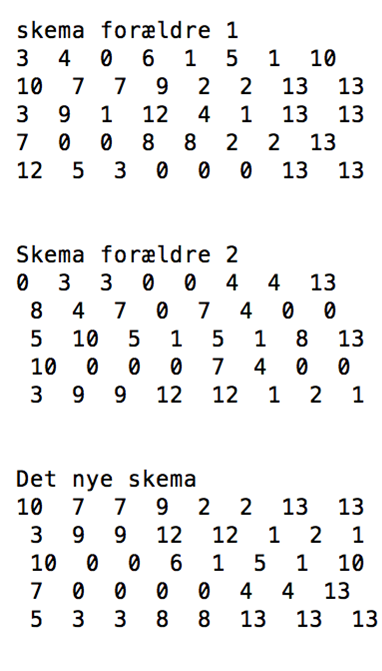
\includegraphics[scale=0.8]{partials/graphics/crossovertest.png}
  \caption{to parents og et child}
  \label{fig:crossovertest}
\end{figure}
